\documentclass[a4paper, notitlepage, 11pt]{article}

\usepackage[a4paper, left=17mm, bottom=17mm, right=35mm, top=17mm]{geometry}

% Common include bundle copied from /home/karen/Dropbox/phd/daily.
% Keep this list in sync when you update the daily includes.

% Style and color palette (used by listings, frames, and headings)
\usepackage[table]{xcolor}

% --------------------------------- colours for content categories
% some colours taken from https://latexcolor.com
\definecolor{codecolor}{rgb}{0.94, 0.92, 0.84}
\definecolor{codeframe}{rgb}{0.84, 0.79, 0.69}
\definecolor{bright_green}{rgb}{0.5, 1.0, 0.0}
\definecolor{amber}{rgb}{1.0, 0.75, 0.0}
\definecolor{brickred}{rgb}{0.8, 0.25, 0.33}
\definecolor{bostonuniversityred}{rgb}{0.8, 0.0, 0.0}
\definecolor{carminered}{rgb}{1.0, 0.0, 0.22}
\definecolor{awesome}{rgb}{1.0, 0.13, 0.32}
\definecolor{darkpastelpurple}{rgb}{0.59, 0.44, 0.84}
\definecolor{titleblue}{rgb}{0.2, 0.2, 0.6}
\definecolor{blush}{rgb}{0.87, 0.36, 0.51}

% set faint color workaround
\colorlet{highlight}{yellow!25}
\colorlet{objective}{carminered!35}
\colorlet{derivation}{pink!50}
\colorlet{grey}{gray!10}
\colorlet{basics}{gray!20}
\colorlet{information}{darkpastelpurple!25}
\colorlet{definition}{orange!10!yellow!30}
\colorlet{surprising}{blue!20}
\colorlet{conclusion}{cyan!20}
\colorlet{donecolor}{cyan!10}
\colorlet{method}{orange!30}
\colorlet{reference}{green!15}

\colorlet{mecolor}{bright_green!50}
\colorlet{roamcolor}{brown!20}
\colorlet{plancolor}{amber!15}
\colorlet{sepiacolor}{darkpastelpurple!20}
% ----------------------- highlighting
\usepackage{soul}
\sethlcolor{highlight}
\DeclareRobustCommand{\hlobj}[1]{{\sethlcolor{objective}\hl{#1}}}
\DeclareRobustCommand{\hlred}[1]{{\sethlcolor{objective}\hl{#1}}}
\DeclareRobustCommand{\hlpink}[1]{{\sethlcolor{derivation}\hl{#1}}}
\DeclareRobustCommand{\hlderiv}[1]{{\sethlcolor{derivation}\hl{#1}}}
\DeclareRobustCommand{\hlgen}[1]{{\sethlcolor{basics}\hl{#1}}}
\DeclareRobustCommand{\hlgrey}[1]{{\sethlcolor{basics}\hl{#1}}}
\DeclareRobustCommand{\ai}[1]{{\sethlcolor{grey}\hl{#1}}}
\DeclareRobustCommand{\hldef}[1]{{\sethlcolor{definition}\hl{#1}}}
\DeclareRobustCommand{\hlyellow}[1]{{\sethlcolor{definition}\hl{#1}}}
\DeclareRobustCommand{\hlaha}[1]{{\sethlcolor{surprising}\hl{#1}}}
\DeclareRobustCommand{\hlpurple}[1]{{\sethlcolor{surprising}\hl{#1}}}
\DeclareRobustCommand{\hlcon}[1]{{\sethlcolor{conclusion}\hl{#1}}}
\DeclareRobustCommand{\hlblue}[1]{{\sethlcolor{conclusion}\hl{#1}}}
\DeclareRobustCommand{\hlmth}[1]{{\sethlcolor{method}\hl{#1}}}
\DeclareRobustCommand{\hlorange}[1]{{\sethlcolor{method}\hl{#1}}}
\DeclareRobustCommand{\hlref}[1]{{\sethlcolor{reference}\hl{#1}}}
\DeclareRobustCommand{\hlgreen}[1]{{\sethlcolor{reference}\hl{#1}}}

\DeclareRobustCommand{\hlcyan}[1]{{\sethlcolor{conclusion}\hl{#1}}}
\DeclareRobustCommand{\hlcode}[1]{{\sethlcolor{codecolor}\hl{#1}}}
\DeclareRobustCommand{\hlme}[1]{{\sethlcolor{mecolor}\hl{#1}}}


% Fonts, unicode support, layout helpers, and general packages
%\usepackage[numbers, sort&compress, square]{natbib}

% bib defintions moved back to master.tex
%\usepackage[backend=biber, natbib=true, sorting=none, style=numeric]{biblatex}
%\usepackage[backend=biber, natbib=true, style=apa]{biblatex}
%\addbibresource{refs.bib}

\usepackage{fontspec}
\defaultfontfeatures{Ligatures=TeX}
% ------------------------------ setting up text fonts with Unicode coverage
\setmainfont{DejaVu Sans}[
	Scale=MatchLowercase,
	BoldFont = DejaVu Sans,
	BoldFeatures = {FakeBold=1.2},
	ItalicFont = DejaVu Sans Oblique,
	BoldItalicFont = DejaVu Sans Oblique,
	BoldItalicFeatures = {FakeBold=1.2}
]
\setsansfont{DejaVu Sans}[
	Scale=MatchLowercase,
	BoldFont = DejaVu Sans,
	BoldFeatures = {FakeBold=1.2},
	ItalicFont = DejaVu Sans Oblique,
	BoldItalicFont = DejaVu Sans Oblique,
	BoldItalicFeatures = {FakeBold=1.2}
]
\renewcommand{\familydefault}{\sfdefault} % sets default document font to sans serif


% ----------------------------- setting up math fonts

\usepackage{amsmath, amssymb, amsthm}
\usepackage{amsfonts}
\usepackage{mathtools}
\PassOptionsToPackage{warnings-off={mathtools-colon,mathtools-overbracket}}{unicode-math}
\usepackage{unicode-math}
\usepackage{mathrsfs}
\setmathfont[Scale=0.89]{Fira Math}
% Fira Math lacks a few symbols used in notes; fallback to Latin Modern for these glyphs.
% TODO: revisit if Fira Math adds these glyphs.
\setmathfont[Scale=0.89]{Latin Modern Math}[range={"225D,"22A4,"22A5,"22EE,"22F1}]
% Use Computer Modern-like alphabets for calligraphic/script/Fraktur and \Im.
\setmathfont[Scale=0.89]{Latin Modern Math}[range=\mathcal]
\setmathfont[Scale=0.89]{Latin Modern Math}[range=\symcal]
\setmathfont[Scale=0.89]{Latin Modern Math}[range=\mathfrak]
\setmathfont[Scale=0.89]{Latin Modern Math}[range=\symfrak]
\setmathfont[Scale=0.89]{Latin Modern Math}[range=\Im]
% Use RSFS for script letters to keep \mathscr visually distinct.
\DeclareSymbolFont{rsfs}{U}{rsfs}{m}{n}
\DeclareSymbolFontAlphabet{\mathscr}{rsfs}

% ------------------------------ setting up monospace font
\setmonofont[
	Scale=0.9,
	BoldFont = * Bold,
	ItalicFont = * Italic,
	BoldItalicFont = * Bold Italic
]{JetBrains Mono}

\newfontfamily\nerdicons{JetBrainsMono Nerd Font}[Scale=MatchLowercase]
\newfontfamily\codeblockfont{JetBrainsMono Nerd Font}[Scale=0.81]

% ------------------------------ FiraFonts
% https://github.com/matze/mtheme/issues/349#issuecomment-648055535
%\usepackage[sfdefault]{FiraSans}
%\usepackage{FiraMono}
% Use thinner fonts
\makeatletter
\def\bfseries@sf{medium}
% DejaVu Sans has no light series; use medium to avoid font warnings.
\def\mdseries@sf{m}
\makeatother

% \usepackage{stix}
%\usepackage[utf8]{inputenc}

% ------------------------------ title format
\usepackage{titlesec}
\titleformat*{\section}{\normalfont\sffamily\bfseries\fontsize{12}{15}\selectfont\color{titleblue}}
\titleformat*{\subsection}{\normalfont\sffamily\bfseries\fontsize{11}{14}\selectfont\color{titleblue}}
\titleformat*{\subsubsection}{\normalfont\sffamily\bfseries\fontsize{10}{13}\selectfont\color{titleblue}}

\usepackage{tocloft} % customise the table of contents


\usepackage{tikz-cd}
\usepackage{markdown}

% --------------------- hyper links
\usepackage{hyperref}
\pdfstringdefDisableCommands{%
	\def\mid{|}%
	\def\alpha{𝛼}%
	\def\Delta{Δ}%
	\def\delta{δ}%
	\def\mathcal#1{#1}%
	\def\mathbb#1{#1}%
	\def\mathrm#1{#1}%
	\def\argmax{\textup{argmax}\ }%
	\def\quad{ }%
}
\hypersetup{
	colorlinks=true,
	linkcolor=black,
	citecolor=black,
	breaklinks=true,
	% subsection depth: paragraph-level bookmarks trigger hyperref
	% bookmark-level warnings at the model section's \paragraph headings
	bookmarksdepth=2,
	hypertexnames=false
}


%\let\hrefori\href%
%\renewcommand{\href}[2]{\hrefori{#1}{\hl{#2}}}

% --------------------- figure support
% graphics and figures
\usepackage{graphicx} % include graphics
\usepackage[export]{adjustbox} % to vertically align figures
\usepackage{wrapfig}
\usepackage{svg}

% subfigures
\usepackage{subcaption}
\renewcommand{\thesubfigure}{\Alph{subfigure}}

\usepackage{import}
\usepackage[shortlabels]{enumitem}
\usepackage{xifthen}
\usepackage{newunicodechar}

\usepackage{pdfpages}
\usepackage{transparent}
\newcommand{\incfigroot}[1]{%
	\def\svgwidth{\columnwidth}
	\import{./}{#1.svg}
}

\usepackage[font=small,labelfont=bf]{caption}
\captionsetup{justification=raggedright,singlelinecheck=false}
% \pdfminorversion=7 % this doesn't work in lualatex
% \pdfsuppresswarningpagegroup=1

\usepackage{parskip}

\newunicodechar{−}{\ensuremath{-}}
\newunicodechar{}{{\nerdicons\symbol{"F023}}}
\newunicodechar{}{{\nerdicons\symbol{"E0B1}}}

% ----------------------- verbatim text like ` in markdown
\usepackage{fancyvrb}
\VerbatimFootnotes%       enable use of \Verb in footnotes
%                         for code use listings package
%\fvset{fontsize=\footnotesize\ttfamily}
\makeatletter
\def\verbatim@font{\ttfamily\small} % block verbatim (\begin{verbatim} …)
\def\verb@font{\ttfamily\small}      % inline \verb|…|
\makeatother



\usepackage{xpatch}
\usepackage{realboxes}
\makeatletter
\xpretocmd\lstinline{\Colorbox{codecolor}\bgroup\appto\lst@DeInit{\egroup}}{}{}
\makeatother


% ----------------------- quoting left bar
\newcommand{\blockquote}[1]{%
	\hspace{0.5em}\begin{tabular}{|p{0.95\textwidth}}#1% chktex 44
	\end{tabular} \par

}

% ----------------------- tcolorbox
\usepackage{tcolorbox}

\tcbset{colframe=blue!25!black,colback=white!95!blue,colupper=blue!25!black,
	fonttitle=\bfseries,nobeforeafter,center title}

% ----------------------------------------   working with dates
\usepackage[en-UK]{datetime2}

% ----------------------------------------  horizontal rule
\newcommand{\widerule}{\noindent\makebox[\textwidth][c]{\rule{0.85\paperwidth}{0.4pt}}}
\newcommand\grayrule{{\color{gray} \noindent\makebox[\linewidth]{\rule{\paperwidth}{0.4pt}}}}


% Code listings configuration (depends on includes-colours)
% listings package configuration
\usepackage{listings}
\usepackage{fvextra}
\usepackage{luacolor}
\usepackage{lua-ul}
%                         https://tex.stackexchange.com/a/466224/151207

%\usepackage{xcolor} % Required for color definitions
% see includes-colours.tex

% Define custom colors
\definecolor{keywordcolor}{rgb}{0.13,0.29,0.53}
\definecolor{stringcolor}{rgb}{0.31,0.60,0.02}
\definecolor{commentcolor}{rgb}{0.56,0.35,0.01}
\definecolor{backcolor}{rgb}{0.95,0.95,0.92}

\definecolor{codecolor}{rgb}{0.94, 0.92, 0.84} % default code background colour
\definecolor{codeframe}{rgb}{0.84, 0.79, 0.69} % default code frame colour

% Julia language definition
\lstdefinelanguage{Julia}{
	basicstyle=\linespread{3}\fontsize{7}{9}\selectfont\fontspec{Fira Code},
	keywordsprefix=\@,
	morekeywords={
			exit,whos,edit,load,is,isa,isequal,typeof,tuple,ntuple,uid,hash,finalizer,convert,promote,
			subtype,typemin,typemax,realmin,realmax,sizeof,eps,promote_type,method_exists,applicable,
			invoke,dlopen,dlsym,system,error,throw,assert,new,Inf,Nan,pi,im,begin,while,for,in,return,
			break,continue,macro,quote,let,if,elseif,else,try,catch,end,bitstype,ccall,do,using,module,
			import,export,importall,baremodule,immutable,local,global,const,Bool,Int,Int8,Int16,Int32,
			Int64,Uint,Uint8,Uint16,Uint32,Uint64,Float32,Float64,Complex64,Complex128,Any,Nothing,None,
			function,type,typealias,abstract},
	sensitive=true,
	alsoother={$},
	morecomment=[l]{\#},
	morecomment=[s]{/*}{*/},
	morestring=[b]",
	morestring=[b]',
}

% General listings settings
\lstset{% 
	basicstyle=\linespread{1.3}\footnotesize\ttfamily,      % font size, mono font, 
	% linespread fixes white tripes
	backgroundcolor=\color{codecolor},  % background color
	showspaces=false,              % show spaces (with underscores)
	frame=single,                  % adds a frame around the code
	tabsize=2,                     % default tabsize
	breaklines=true,               % automatic line breaking
	columns=fullflexible,
	framerule=0.5pt,
	rulecolor=\color{codeframe},
	framesep=1em,                  % padding
	xleftmargin=1em,
	columns=fullflexible,          % make sure to use fixed-width font, CM typewriter is NOT fixed width
	numbers=none,                  % left
	numberstyle=\footnotesize\ttfamily\color{codeframe},
	numbersep=5pt,                 % how far the line numbers are from the code
	stepnumber=1,
	numberfirstline=true,
	numberblanklines=true,
	tabsize=4,
	lineskip=-1.5pt,
	extendedchars=true,
	mathescape=false,
	breaklines=true,
	keywordstyle=\color{keywordcolor}\bfseries,
	identifierstyle=, % using emph or index keywords
	commentstyle=\color{commentcolor},
	stringstyle=\color{stringcolor},
	showstringspaces=false,
	showtabs=false,
	upquote=false,
	%texcl=true, % interpet comments as LaTeX
	literate={_}{\_}1
}

% Robust inline code.  This uses fvextra's verbatim reader rather than wrapping
% \lstinline in another macro, so raw underscores and long paths are safe.
% commandchars keeps legacy notes such as \code{foo\_bar} readable.
% Paper style: inline code as plain typewriter, no highlight background
\renewcommand{\FancyVerbFormatInline}[1]{#1}
\newcommand{\code}{\Verb[
	breaklines=true,
	breakanywhere=true,
	breaksymbolleft={},
	breaksymbolright={},
	formatcom=\codeblockfont\small,
	commandchars=\\\{\}
]}
\pdfstringdefDisableCommands{%
	\def\code#1{#1}%
}

% Plain verbatim blocks. Keep this on FancyVerb/fvextra rather than listings:
% listings inline state can leak into aux/toc writes in recent TeX Live.
\makeatletter
\define@key{FV}{plancolor}[]{\fvset{bgcolor=plancolor,fillcolor=\color{plancolor}}}
\define@key{FV}{robocupcolor}[]{\fvset{bgcolor=robocupcolor,fillcolor=\color{robocupcolor}}}
\define@key{FV}{sepiacolor}[]{\fvset{bgcolor=sepiacolor,fillcolor=\color{sepiacolor}}}
\define@key{FV}{donecolor}[]{\fvset{bgcolor=donecolor,fillcolor=\color{donecolor}}}
\makeatother
\DefineVerbatimEnvironment{lstplain}{Verbatim}{
	fontsize=\scriptsize,
	baselinestretch=0.95,
	formatcom=\codeblockfont,
	breaklines=true,
	breakanywhere=true,
	breaksymbolleft={},
	breaksymbolright={},
	bgcolor=codecolor,
	frame=single,
	framerule=0.5pt,
	framesep=1em,
	xleftmargin=0em,
	rulecolor=\color{codeframe},
	fillcolor=\color{codecolor}
}

\DefineVerbatimEnvironment{vrb}{Verbatim}{
	fontsize=\scriptsize,
	baselinestretch=0.95,
	formatcom=\codeblockfont,
	breaklines=true,
	breakanywhere=true,
	breaksymbolleft={},
	breaksymbolright={},
	bgcolor=codecolor,
	frame=single,
	framerule=0.5pt,
	framesep=1em,
	xleftmargin=0em,
	rulecolor=\color{codeframe},
	fillcolor=\color{codecolor}
}


\lstnewenvironment{lstjulia}[1][codecolor]{
	\lstset{% 
		language=Julia,
		basicstyle=\fontsize{7}{9}\selectfont\fontspec{Fira Code},
		xleftmargin=0em,
		backgroundcolor=\color{#1},
		commentstyle=\color{commentcolor},
		keywordstyle=\color{keywordcolor},
		stringstyle=\color{stringcolor},
		numberstyle=\tiny\color{gray},
		breaklines=true,
		showstringspaces=false,
		frame=single,
		tabsize=2,
		literate={_}{\_}1
	}
}{}

\lstnewenvironment{lstpython}[1][codecolor]{
	\lstset{%
		language=Python,
		basicstyle=\fontsize{7}{9}\selectfont\fontspec{Fira Code},
		xleftmargin=0em,
		backgroundcolor=\color{#1},
		commentstyle=\color{commentcolor},
		keywordstyle=\color{keywordcolor},
		stringstyle=\color{stringcolor},
		numberstyle=\tiny\color{gray},
		breaklines=true,
		showstringspaces=false,
		frame=single,
		tabsize=2,
		literate={_}{\_}1
	}
}{}


% Math and symbols
% ------------------------------ define equals
% also \coloneqq and \eqqcolon from mathtools imported below
\newcommand{\defeq}{\vcentcolon=}
\newcommand{\eqdef}{=\vcentcolon}

% ------------------------------ Expectation, Var and Covar symbol
% when declaring math operators the * denotes the use of limits above and/or below
\DeclareMathOperator*{\E}{\mathbb{E}}
\DeclareMathOperator*{\Var}{\operatorname{Var}}
\DeclareMathOperator*{\Cov}{\operatorname{Cov}}


% ----------------------------- set complement
\newcommand{\stcomp}[1]{{#1}^{\mathsf{c}}}
% ----------------------------- argmax and argmin
\DeclareMathOperator*{\argmax}{arg\,max\,}
\DeclareMathOperator*{\argmin}{arg\,min\,}

% ----------------------------- transpose and other matrix notation
% https://tex.stackexchange.com/a/217623/151207
% unicode-math not supported in pdftex
% \usepackage{mathtools} % in preamble
%\usepackage{unicode-math}
\newcommand*{\matr}[1]{\mathbf{#1}}
\newcommand*{\tran}{^{\mkern-1.5mu\mathsf{T}}}
\newcommand*{\conj}[1]{\overline{#1}}
\newcommand*{\hermconj}{^{\mathsf{H}}}
% trace of a matrix
\DeclareMathOperator{\Tr}{Tr}
% cardinality of a matrix and vector
\newcommand{\matdim}[2]{\mathsf{\textit{#1}\times\textit{#2}}}
\newcommand{\vecdim}[1]{\mathsf{\textit{#1}}}

% Define a command for a placeholder matrix with dimensions m x n
\newcommand{\matblock}[3]{
	\begin{bmatrix}
		#1_{\mathsf{\textit{1,1}}}  & \cdots & #1_{\mathsf{\textit{1,#3}}}  \\
		\vdots                      & \ddots & \vdots                       \\
		#1_{\mathsf{\textit{#2,1}}} & \cdots & #1_{\mathsf{\textit{#2,#3}}}
	\end{bmatrix}
}

% Define a command for a placeholder vector with dimension m
\newcommand{\vecblock}[2]{
	\begin{bmatrix}
		#1_{\mathsf{\textit{1}}} \\
		\vdots                   \\
		#1_{\mathsf{\textit{#2}}}
	\end{bmatrix}
}

\newcommand{\C}{\mathbb{C}}
\newcommand{\R}{\mathbb{R}}
\newcommand{\Q}{\mathbb{Q}}
\newcommand{\Z}{\mathbb{Z}}
\renewcommand{\L}{\mathcal{L}}
% ...
% Information to go symbol
\usepackage{scalerel}    % required for scaleto
% Information-to-go symbol (bold imaginary unit)
\newcommand{\Itg}{\ensuremath{\pmb{\Im}}}
% Decision information symbol
\newcommand{\ItgD}{\ensuremath{\pmb{\symcal{I}}}}
% Environmental response / empowerment-like information
\newcommand{\ItgE}{\ensuremath{\pmb{\symcal{E}}}}
% empowerment (maximised over policies)
\newcommand{\emp}{\ensuremath{\mathfrak{E}}}

% Uniform distribution
\newcommand{\U}{\ensuremath{\mathrm{U}}}

% Action/state set symbols
\renewcommand{\S}{\ensuremath{\mathcal{S}}}
\newcommand{\A}{\ensuremath{\mathcal{A}}}

% Free energy and policy notation
\newcommand{\Fen}{\ensuremath{\pmb{\symcal{F}}}}
\newcommand{\pif}{{\ensuremath{\pi_{\scaleto{\Fen}{3pt}}}}}
\newcommand{\piv}{{\ensuremath{\pi_{\scaleto{V}{3pt}}}}}
% Leg subpolicies and glued composite (space-of-goals sup-matl convention)
\newcommand{\pifi}[1]{{\ensuremath{\pi_{\scaleto{\Fen}{3pt}}^{\scaleto{(#1)}{4pt}}}}}
\newcommand{\pifhat}{{\ensuremath{\hat{\pi}_{\scaleto{\Fen}{3pt}}}}}
% Triangle-inequality defect: composite (legs) minus direct.
% Paper / epsilon-infodesic sign:  \dFen < 0  <=>  switching helps (deficiency).
\newcommand{\dFen}{\ensuremath{\Delta\Fen}}
% mu-referenced open-loop action marginal (January reworking): \phatmu(a)=sum_s mu(s) pi(a|s)
\newcommand{\phatmu}{\ensuremath{\hat p^{\mu}}}

% Short arrow symbols used for action sets (copied from progression-report includes-preamble).
\usepackage{stmaryrd}
\makeatletter
\newcommand{\fixed@sra}{$\vrule height 2\fontdimen22\textfont2 width 0pt\shortrightarrow$}
\newcommand{\shortarrow}[1]{%
  \mathrel{\text{\rotatebox[origin=c]{\numexpr#1*45}{\fixed@sra}}}
}
\makeatother


% Framed environments and references
\usepackage{mdframed}
\mdfsetup{
	leftmargin=-1em,
	rightmargin=-1em,
	middlelinewidth=1.5pt,
	middlelinecolor=white,
	innertopmargin=\topskip,
	innerbottommargin=.50\topskip,
	skipabove=0.5\baselineskip,
	skipbelow=0,
	nobreak=true
}

\newmdenv[
	backgroundcolor = red!10
]{wrong}

\newmdenv[
	backgroundcolor = green!10
]{correct}

% colours
\colorlet{vlcolor}{brown!15}
\definecolor{unired}{rgb}{0.8, 0.0, 0.0}
\colorlet{coursescolor}{unired!15}
\colorlet{robocupcolor}{lime!20}
\colorlet{stridecolor}{lime!30}

% frames to colour code topics
% phd - all the following activities relate to my phd
% problem
% reading
% coding
% thinking
% question
% answer - never used
% course - change to learning?
% vl
% robocup
% writing
% todo


\newmdtheoremenv[backgroundcolor=cyan!30]{answer}{Answer}[section]

\newmdtheoremenv[backgroundcolor=coursescolor]{course}{Course}[section]
\newmdtheoremenv[backgroundcolor=coursescolor]{learning}{Learning}[section]
\newmdtheoremenv[backgroundcolor=orange!20]{problem}{Problem}[section]

% TODO heading style: bold title with optional short heading (no parentheses).
\newtheoremstyle{todostyle}%
	{0.5\baselineskip}{0.5\baselineskip}%
	{\normalfont}{}%
	{\normalfont\sffamily\color{titleblue}}%
	{.}{0.5em}%
	{\thmname{#1}\thmnote{ -- #3}}
\theoremstyle{todostyle}
\newmdtheoremenv[backgroundcolor=cyan!20]{todo}{TODO}
\renewcommand{\thetodo}{} % remove numbering from todo
\theoremstyle{definition}

\newmdtheoremenv[backgroundcolor=cyan!15]{done}{Working}[section]

\newcommand{\frameheading}[2]{%
	{\color{titleblue}\sffamily\bfseries\fontsize{11}{14}\selectfont #1: \textsection\thesection\hspace{1em}#2}%
}

\newmdenv[backgroundcolor=mecolor!40,nobreak=false]{phd}
\newcommand{\phdsec}[1]{%
	\refstepcounter{section}
	\addcontentsline{toc}{section}{\thesection\hspace{1em}PhD: #1}
	\begin{phd}\frameheading{PhD}{#1}\end{phd}
}

\newmdtheoremenv[backgroundcolor=coursescolor]{research}{Research}
\newcommand{\researchsec}[1]{%
	\refstepcounter{section}
	\addcontentsline{toc}{section}{\thesection\hspace{1em}Research: #1}
	\begin{research}\frameheading{Research}{#1}\end{research}
}

\newmdenv[backgroundcolor=mecolor]{coding}
\newcommand{\codingsec}[1]{%
	\refstepcounter{section}
	\addcontentsline{toc}{section}{\thesection\hspace{1em}Coding: #1}
	\begin{coding}\frameheading{Coding}{#1}\end{coding}
}

\newmdenv[backgroundcolor=green!10,nobreak=false]{reading}
\newcommand{\readingsec}[1]{%
	\refstepcounter{section}
	\addcontentsline{toc}{section}{\thesection\hspace{1em}Reading: #1}
	\begin{reading}\frameheading{Reading}{#1}\end{reading}
}

\newmdenv[backgroundcolor=blue!20,nobreak=false]{thinking}
\newcommand{\thinkingsec}[1]{%
	\refstepcounter{section}
	\addcontentsline{toc}{section}{\thesection\hspace{1em}Thinking: #1}
	\begin{thinking}\frameheading{Thinking}{#1}\end{thinking}
}

\newmdenv[backgroundcolor=cyan!10]{meeting}
\newcommand{\meetingsec}[1]{%
	\refstepcounter{section}
	\addcontentsline{toc}{section}{\thesection\hspace{1em}Meeting: #1}
	\begin{meeting}\frameheading{Meeting}{#1}\end{meeting}
}

\newmdenv[backgroundcolor=green!30,nobreak=false]{question}
\newcommand{\questionsec}[1]{%
	\refstepcounter{section}
	\addcontentsline{toc}{section}{\thesection\hspace{1em}Question: #1}
	\begin{question}\frameheading{Question}{#1}\end{question}
}

\newmdenv[backgroundcolor=darkpastelpurple!25,nobreak=false]{workflow}
\newcommand{\workflowsec}[1]{%
	\refstepcounter{section}
	\addcontentsline{toc}{section}{\thesection\hspace{1em}Workflow: #1}
	\begin{workflow}\frameheading{Workflow}{#1}\end{workflow}
}

\newmdenv[backgroundcolor=stridecolor, nobreak=false]{stride}
\newcommand{\stridesec}[1]{%
	\refstepcounter{section}
	\addcontentsline{toc}{section}{\thesection\hspace{1em}stride: #1}
	\begin{stride}\frameheading{STRIDE}{#1}\end{stride}
}

\newmdenv[backgroundcolor=robocupcolor, nobreak=false]{robocup}
\newcommand{\robocupsec}[1]{%
	\refstepcounter{section}
	\addcontentsline{toc}{section}{\thesection\hspace{1em}Robocup: #1}
	\begin{robocup}\frameheading{Robocup}{#1}\end{robocup}
}

\newmdenv[backgroundcolor=robocupcolor, nobreak=false]{rl}
\newcommand{\rlsec}[1]{%
	\refstepcounter{section}
	\addcontentsline{toc}{section}{\thesection\hspace{1em}RL: #1}
	\begin{rl}\frameheading{RL}{#1}\end{rl}
}

\newmdtheoremenv[backgroundcolor=vlcolor]{vl}{VL}
\newcommand{\vlsec}[1]{%
	\refstepcounter{section}
	\addcontentsline{toc}{section}{\thesection\hspace{1em}VL: #1}
	\begin{vl}\frameheading{VL}{#1}\end{vl}
}

\newmdtheoremenv[backgroundcolor=vlcolor]{writing}{WRITING}
\newcommand{\writingsec}[1]{%
	\refstepcounter{section}
	\addcontentsline{toc}{section}{\thesection\hspace{1em}WRITING: #1}
	\begin{writing}\frameheading{writing}{#1}\end{writing}
}



\newmdenv[backgroundcolor=roamcolor, nobreak=false]{roam}
\newcommand{\roamsec}[1]{%
	\refstepcounter{section}
	\addcontentsline{toc}{section}{\thesection\hspace{1em}Roam: #1}
	\begin{roam}\frameheading{Roam}{#1}\end{roam}
}

\newmdenv[backgroundcolor=roamcolor, nobreak=false]{topic}
\newcommand{\topicsec}[1]{%
	\refstepcounter{section}
	\addcontentsline{toc}{section}{\thesection\hspace{1em}Topic: #1}
	\begin{topic}\frameheading{Topic}{#1}\end{topic}
}

%\newmdtheoremenv[backgroundcolor=lime!40]{section}{\thesection\hspace{1em}Robocup: #1}

%\usepackage{hyperref}
%\hypersetup{hidelinks}
\usepackage{fontawesome}
\usepackage{xifthen}% provides \isempty test
\Urlmuskip=0mu plus 2mu\relax
\newcommand\pdfref[3]{%
    \href{phd://open-paper?id=#1&page=#2}{%
    \textup{[\ifthenelse{\isempty{#3}}{here}{#3}]}}%
}

\newcommand\urlref[2]{%
    \href{#1}{\raisebox{0.15ex}{\scriptsize \faLink}\:\textup{#2}}%
}

% \newcommand\urlref[2]{%
%     \def\argone{#1} % Store the first argument (URL) in \argone
%     \def\argtwo{#2} % Store the second argument (label) in \argtwo
% 
%     % Check if \argone is empty
%     \ifx\argtwo\@empty
%         \edef\argone{#1} % If \argone is empty, use \argtwo as URL
%         \edef\argtwo{#1} % And use \argtwo for both URL and label
%     \fi
%     \href{\argone}{\raisebox{0.15ex}{\scriptsize \faLink}\:\textup{\textbf{\argtwo}}}%
% }

\newcommand{\dailyfilelabel}[1]{%
    {\footnotesize\nolinkurl{#1}}%
}

\newcommand\absolutefileref[2]{%
    \href{run:#1}{\raisebox{0.15ex}{\scriptsize \faFile}\:\textup{#2}}%
}

% this will contain the current date in yyyy-mm-dd format
\def\formatteddate{}
\newcommand\fileref[2]{
    \IfFileExists{./\formatteddate/#1}{
        \absolutefileref{./\formatteddate/#1}{#2}
    }{
        \textcolor{gray}{\absolutefileref{./\formatteddate/#1}{#2}}
    }
}
 
% daily path reference
\newcommand{\dailypath}{.\formatteddate\monthFolder\dayFolder}


% daily file reference
\newcommand{\dailyfileref}[1]{%
  \fileref{\dailypath/#1}{\dailyfilelabel{#1}}%
}

% daily include graphic
\newcommand{\fig}[1]{%
  \includegraphics[width=0.98\textwidth]{\dailypath/#1}%
}

% daily include graphic with adjustable width
\newcommand{\figw}[2]{%
  \includegraphics[width=#2\textwidth]{\dailypath/#1}%
}

%\newcommand{\xournal}{\fileref{note.xopp}{Handwritten notes}}%

%\newcommand{\pdfnotes}{\fileref{\monthFolder/\dayFolder/note.pdf}{Handwritten notes}}%


% Table of contents styling and table helpers
% adjusting the formatting for the phantom sections / parts in the toc
\setlength{\cftbeforepartskip}{0.5em}  % adjust the spacing before
\setlength{\cftbeforesecskip}{0.5em}  % adjust the spacing before

% widen the number boxes so multi-digit section numbers don't collide with titles
\setlength{\cftsecnumwidth}{3.2em}
\setlength{\cftsubsecnumwidth}{3.8em}
\setlength{\cftsubsubsecnumwidth}{4.4em}

% adjusting font size and font series for different content types
\renewcommand{\cftpartfont}{\small\bfseries} % part 
\renewcommand{\cftsecfont}{\small\sffamily}
\renewcommand{\cftsubsecfont}{\small\sffamily}
\renewcommand{\cftsubsubsecfont}{\footnotesize\sffamily}

% change the font size of the page numbers for various content types
\renewcommand{\cftpartpagefont}{\small}          %  part page numbers
\renewcommand{\cftsecpagefont}{\small}           %  section page numbers
\renewcommand{\cftsubsecpagefont}{\small}        %  subsection page number
\renewcommand{\cftsubsubsecpagefont}{\footnotesize}     %  subsubsection page number

\cftpagenumbersoff{subsubsection}

% for a solid leader line 
% define custom line fill
\newcommand{\cftlinefill}[1]{%
	\leavevmode\leaders\hrule height #1\hfill\kern0.5em
}

% Leader lines 
\renewcommand{\cftpartleader}{{\color{gray}\cftlinefill{0.1pt}}}
%\renewcommand{\cftpartleader}{\cftdotfill{\cftdotsep}} % Use dot leaders for parts
\renewcommand{\cftsecleader}{{\cftlinefill{0.1pt}}}
\renewcommand{\cftsubsecleader}{\hfill}
\renewcommand{\cftsubsubsecleader}{\hfill}



% Define a new counter for days
\newcounter{daycount}
\setcounter{daycount}{0}

\newcommand{\daymarker}[1]{%
	% Use the provided date shorthand to format the date
	% Assuming #1 is a formatted string using PGF/TikZ date tools
	% example usage 
	%     \daymarker{\d y0-\d m0-\d d0}
	%     \daymarker{\d wt, \d d0 \d m. }

	\phantomsection % part of hyperref package - creates an anchor without a new section
	\addcontentsline{toc}{part}{#1}
	% Display the marker in the document, if needed
	%\textbf{#1} % Example placement, adjust as necessary
	\ifdate{equals=\firstdate}{}{%
		\bigskip
		\ifdate{Monday}{\grayrule\\[-22pt]\grayrule}{\grayrule}
	}%
	\vspace*{1em}
	\marginpar{\vspace*{1em}\textsf{ \d w., \d m. \d d- }}%
	\stepcounter{daycount} % Increment the day counter
}

\usepackage{tabularx}

\usepackage{colortbl}

\usepackage{makecell}
\usepackage{multirow}
\renewcommand\theadfont{\bfseries}
% Define a new command for left-aligned header cells
\newcommand{\leftthead}[1]{\makecell[l]{#1}}
% change row height for all tables
\renewcommand{\arraystretch}{1.5}

\usepackage{booktabs}
\usepackage{array}

% for use with tabular environment
\newcolumntype{L}[1]{>{\raggedright\let\newline\\\arraybackslash\hspace{0pt}}p{#1}}
\newcolumntype{C}[1]{>{\centering\let\newline\\\arraybackslash\hspace{0pt}}p{#1}}
\newcolumntype{R}[1]{>{\raggedleft\let\newline\\\arraybackslash\hspace{0pt}}p{#1}}

% singlelinecheck=false stops the table caption being centered
\captionsetup{singlelinecheck=false}



\newfontfamily\papercodeblockfont{JetBrainsMono Nerd Font}[Scale=MatchLowercase]
\renewcommand{\codeblockfont}{\papercodeblockfont}

\usepackage[backend=biber, natbib=true, style=apa]{biblatex}
\addbibresource{refs.bib}

\usepackage{float}

\graphicspath{{figures/}}

\title{Cheap worlds first:\\ two-stage goal-subsampling annealing for evolving action relabellings}
\author{Karen Archer\textsuperscript{1},\, [co-authors TBC]}
\date{FIRST DRAFT --- 2026-07-09}

\makeatletter
\renewcommand{\@maketitle}{%
  \begin{center}
    {\Large\bfseries \@title \par}
    \vspace{0.75em}
    {\normalsize \@author \par}
    \vspace{0.5em}
    {\small \textsuperscript{1}Adaptive Systems Group, University of Hertfordshire, Hatfield, UK \par}
    \vspace{0.5em}
    {\small \@date \par}
  \end{center}
  \vspace{1em}
}
\makeatother

% ---------------------------------------------------------------------------
% FIRST DRAFT.  All numbers verified against synced run data 2026-07-07/08.
% Sources: gridFour/notebooks/attractor-fingerprint-probe/46,48,49,50,52;
% goal-subsampling-validation/01-03; gridOps/vars manifests; synced runs
% under /media/merlin/grid-twist/gridtwist-outputs/.  25x25 pair pending
% (stage-1 in progress, ETA ~2026-07-14).
% ---------------------------------------------------------------------------

\begin{document}

\maketitle

\begin{abstract}
Evolving per-state action relabellings (\emph{twists}) for multi-goal
navigation is dominated by fitness evaluation: every genome scores as one
planning solve per goal, and the goal set grows with the world.  We show
that a two-stage schedule --- evolve on a $10\%$ random goal subsample,
then consolidate with a short full-goal tail seeded from the stage-one
population --- finds \emph{better} twists than full-goal evolution at a
fraction of the cost, at every environment and scale tested.  On a
$13 \times 13$ walled world the annealed runs beat a five-times-budget
full-goal baseline at $28\%$ of its evaluation cost; at $15 \times 15$,
where fixed-budget full-goal search starves, annealing recovers the homing
structure the baselines lose.  The subsampled stage finds the same
attractor objects, not merely comparable fitness: in a seed-matched pilot
the consolidation tail inherits the stage-one attractor exactly (cycle
Jaccard $1.00$) and completes it in place.  The obvious de-noising
alternative --- re-scoring elite genomes on the full goal set --- is
actively harmful, halving the rate at which runs reach the strong homing
mode.  The subsampling noise is not a defect to be corrected but the
mechanism itself: a cheap, wide search that annealing then sharpens.
\end{abstract}

\section{Introduction}
\label{sec:intro}

A twist assigns each state its own permutation of the action labels,
leaving the world unchanged; evolved twists make multi-goal navigation
informationally cheaper and build \emph{homing labels} --- single labels
whose repeated execution drains large regions of the world into a compact
attractor \citep{Archer2026-relabelled-actions}.  The obstacle to studying
these structures at scale is not the genetic algorithm but its fitness
function.  Multi-goal fitness is a mean over goals, and each goal costs a
full planning solve (a Blahut--Arimoto iteration to convergence): a
population of $96$ evaluated over $200$ generations against every goal of
a $15 \times 15$ walled world is roughly four million solves.  Grid worlds
grow quadratically; goal sets grow with them; the evaluation bill grows as
their product.

The standard responses are surrogate fitness models and fitness
approximation by sampling.  This paper takes the sampling route in its
simplest form and asks the question that matters for structural research:
not \emph{does cheap noisy fitness find something about as good}, but
\emph{does it find the same objects}?  If a goal-subsampled search
discovers different attractor structures --- different homing labels,
different home cycles --- then the saving is a false economy for any
analysis that studies the structures themselves.  If it finds the same
objects, the evaluation bill for an entire research programme drops by a
factor of three or more.

We answer with a two-stage schedule we call \emph{K-annealing}: evolve at
goal-subsample fraction $K = 0.1$ (a fresh random $10\%$ mini-batch of
goals per generation), then anneal to $K = 1$ for a short consolidation
tail whose initial population is the stage-one final population.  Three
results support it.  First, a seed-matched pilot at $9 \times 9$ shows the
tail meets full-goal quality bars while inheriting the stage-one attractor
\emph{exactly} --- same cycle cells, same home --- at $28\%$ of the
full-goal evaluation cost.  Second, the schedule scales: at $13 \times 13$
and $15 \times 15$, on both a heavily walled world and a seamed torus, the
annealed runs beat every seed-matched full-goal baseline we hold,
including one with five times the generation budget.  Third, and most
diagnostic of the mechanism: the obvious refinement of re-scoring elites
on the full goal set each generation \emph{harms} the search, halving the
rate at which runs reach the strong homing mode.  The mini-batch noise is
doing the exploring.

\section{Two-stage K-annealing}
\label{sec:method}

The genetic algorithm is the one used throughout the twists programme
\citep{Archer2026-relabelled-actions}: population $96$, tournament size
$3$, elite size $4$; crossover exchanges whole state-rows with probability
$0.7$, mutation swaps two labels within a row (row probability $0.2$,
genome probability $0.3$), so genomes remain per-state permutations.
Fitness is the mean planning cost over the evaluated goal set --- here
mean free energy $\mathbb{E}_{s,g}[\Fen^{\pi^*_\beta}(s)]$ at $\beta = 1$,
each $(\sigma, g)$ pair solved to $\theta = 10^{-5}$.

\paragraph{Stage one: subsampled evolution.}  At goal-subsample fraction
$K < 1$, each generation draws a fresh uniform mini-batch of
$\lceil K \lvert G \rvert \rceil$ goals and scores every genome against
that batch.  The batch changes every generation and is recorded with the
generation for audit.  Elites are cloned across generations but their
fitness is invalidated and re-scored on each new batch --- an elite
survives only by remaining good on goals it has not been selected on.
Solved $(\sigma, g)$ pairs are cached by twist hash and goal in a
run-local store whose key deliberately excludes $K$, so nothing solved in
stage one is ever re-solved later.

\paragraph{Stage two: the full-goal tail.}  At the end of stage one the
final population --- all $96$ genomes, not the single best --- is written
as a genome array with a provenance sidecar (environment, shape, action
count), and a second, short run starts at $K = 1$ with that array as its
initial population.  The sidecar is validated on load, so a population
cannot silently seed a mismatched world.  Because the evaluation cache is
$K$-agnostic, the tail begins with every stage-one solve already in hand;
its marginal cost is the full-goal evaluation of genuinely new genomes.
Loading a population consumes no random draws, so the tail is a new
evolutionary trajectory, not a replay.

\paragraph{Cost accounting.}  We count cost in \emph{goal-generation
equivalents}: one unit is one generation evaluated against the full goal
set.  A stage-one generation at $K = 0.1$ costs $0.1$ units, so the
schedule used throughout this paper --- $800$ generations at $K = 0.1$
plus a $200$-generation tail at $K = 1$ --- costs $280$ units.  The
baselines it is judged against cost $200$, $500$, and $1{,}000$ units.
Wall-clock tracks these units closely; the pilot's annealed lineages
completed, both stages, in about an hour each on one lab node.

\section{Pilot: same attractor, quarter cost}
\label{sec:pilot}

The pilot ran three seed-matched lineages on \code{four\_rooms}
$9 \times 9$: for each seed, a stage-one run ($K = 0.1$, $g = 800$) and
its tail ($K = 1$, $g = 200$), judged against the seed-matched full-goal
baselines already held for that world.  Two quality bars were set in
advance from those baselines: the tail should reach the baselines' mean
run-best coverage ($0.804$), and ideally their best ($0.838$).

\paragraph{Quality.}  The three tails reached coverage $0.838$, $0.794$,
and $0.838$ (mean $0.823$): two of three hit the historical best outright.
Final best mean free energies were $13.18$, $13.21$, and $13.23$ ---
inside the baseline cluster --- and each tail improved on its own
stage-one final ($13.24$, $13.30$, $13.47$), the consolidation worth
$0.07$--$0.24$ bits.

\paragraph{Identity.}  The claim that matters for structural research is
that stage one finds the \emph{object} and the tail merely completes it.
Comparing each tail's dominant-label functional graph against its own
stage-one final: basin Jaccard $0.89$--$0.95$, attractor-cycle Jaccard
$1.00$ --- identical cycle cells in all three lineages, every cycle
containing the same home cell --- and identical dominant-label dwell
structure.  At the genome level, $84$--$93\%$ of $\sigma$ rows are
byte-identical between a stage-one final and its tail's run-best.  Across
lineages the picture is the familiar stochastic one: all three home in the
same room (cross-lineage basin Jaccard $0.73$--$0.88$) with idiosyncratic
micro-cycles.  The tail does not re-search; it consolidates in place
(Figure~\ref{fig:pilot-overlay}).

\begin{figure}[H]
  \centering
  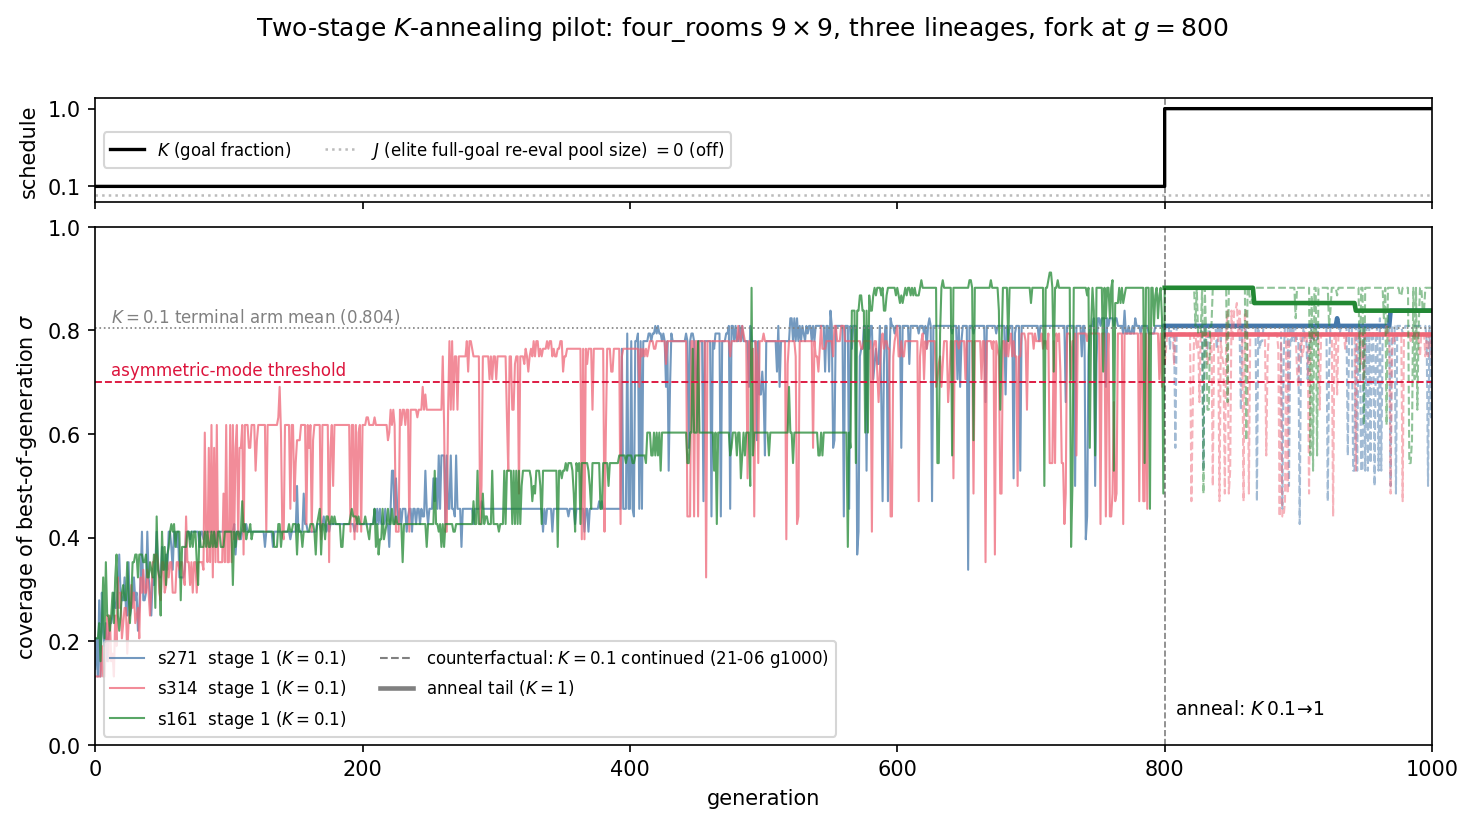
\includegraphics[width=0.98\textwidth]{F-anneal-pilot-trajectory.png}
  \caption[Pilot schedule and coverage fork]{The two-stage schedule on the
  pilot.  The $K$ schedule --- $800$ generations at $K = 0.1$, then the
  $K = 1$ tail seeded from the stage-one population --- with run-best
  coverage along the run and the counterfactual fork: continuing at
  $K = 0.1$ churns without consolidating, while the full-goal tail locks
  in the found structure and completes it.}
  \label{fig:pilot-schedule}
\end{figure}

\begin{figure}[H]
  \centering
  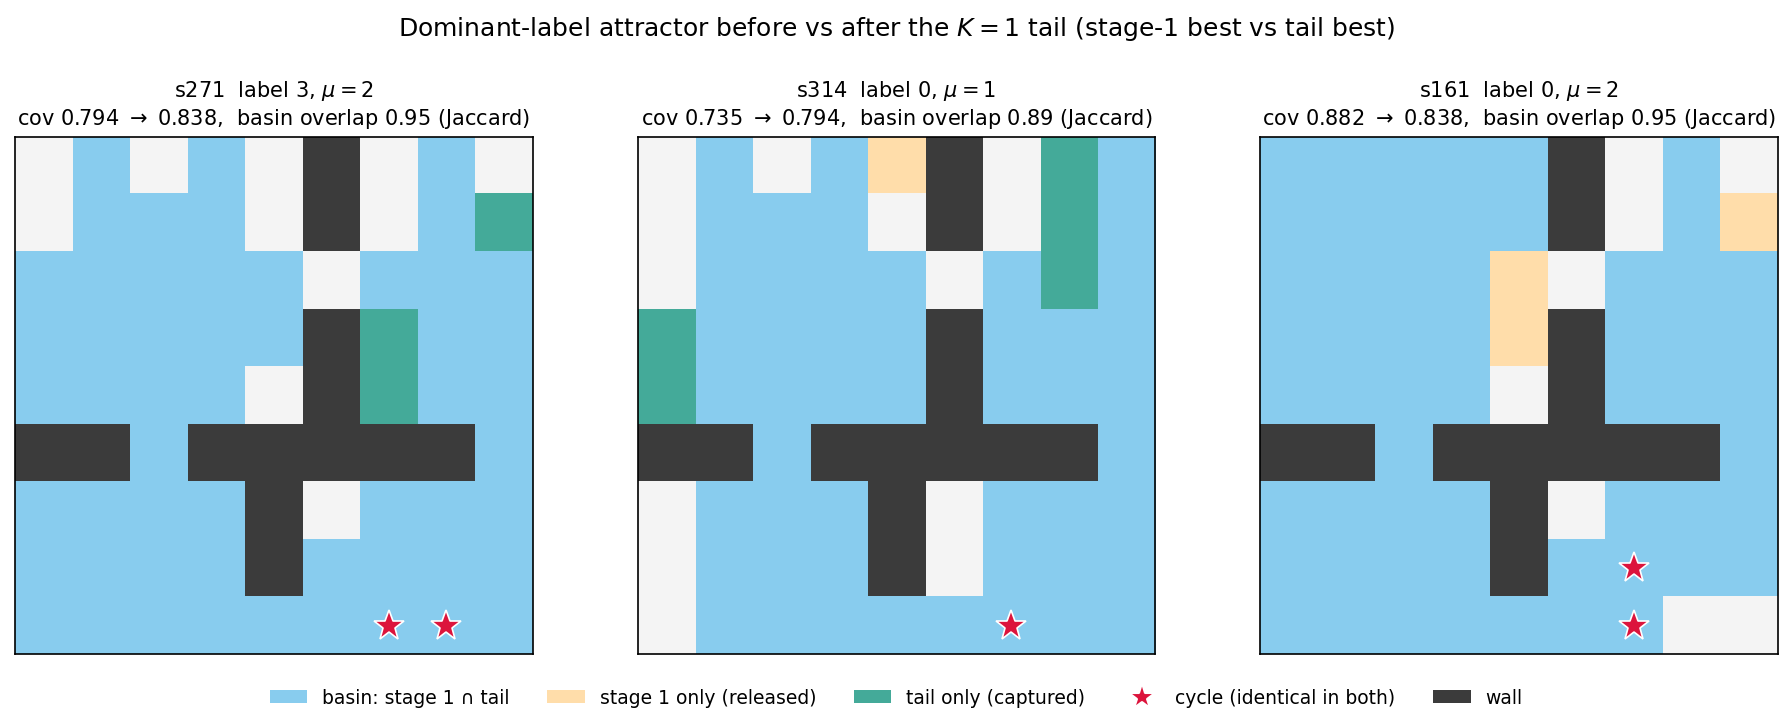
\includegraphics[width=0.9\textwidth]{F-anneal-pilot-attractor-overlay.png}
  \caption[Pilot attractor overlay]{Stage-one final against tail run-best
  for the pilot lineages: the dominant-label basin and its attractor
  cycle.  The tail inherits the attractor exactly --- cycle Jaccard
  $1.00$ in all three lineages --- and tidies the basin margins (basin
  Jaccard $0.89$--$0.95$).}
  \label{fig:pilot-overlay}
\end{figure}

\section{The de-noising trap}
\label{sec:j-harmful}

Mini-batch fitness is noisy, and the obvious refinement is to spend a
little of the saved budget de-noising where it seems to matter most: the
elites.  In this variant, the elite pool is re-scored against the full
goal set each generation, anchoring selection's top end to the true
objective while the population explores cheaply.

It does the opposite of what it promises.  In a four-seed comparison at
$9 \times 9$, plain subsampled evolution reached the strong homing mode
(coverage $\geq 0.70$) in three of four seeds at both $K = 0.1$ and
$K = 0.25$; adding full-goal elite re-evaluation dropped this to one of
four.  Re-scoring the elites re-anchors selection to the current best
full-goal genomes every generation, and the population contracts around
them before the cheap exploration has found the basin worth
consolidating.  The batch noise at the top of the ranking is not a defect:
it is what keeps early, mediocre structure from entrenching.  Selection
pressure in a noisy fitness landscape is itself annealed by the noise, and
the two-stage schedule works precisely because it removes that noise
\emph{once}, at the end, rather than continuously at the top.

\section{Annealing at scale}
\label{sec:scale}

The pilot licenses the schedule; scale is where it pays.  We ran the same
two-stage schedule ($K = 0.1$, $g = 800$; tail $K = 1$, $g = 200$; two
seeds per world) on \code{four\_rooms} at $13 \times 13$ and
$15 \times 15$ and on the seamed torus \code{helical} at $15 \times 15$,
against every seed-matched full-goal baseline we hold.
Table~\ref{tab:scale} gives the complete accounting.

\begin{table}[H]
  \centering
  \small
  \begin{tabular}{llccc}
    \toprule
    world & seed & anneal (stage $\to$ tail) & best $K{=}1$ baseline & cost ratio \\
    \midrule
    \code{four\_rooms} $13{\times}13$ & s141 & $18.55 \to \mathbf{18.48}$ & $18.71$ \; ($g = 1000$) & $0.28$ \\
    \code{four\_rooms} $13{\times}13$ & s223 & $18.68 \to \mathbf{18.56}$ & $19.15$ \; ($g = 200$) & $1.4$ \\
    \code{four\_rooms} $15{\times}15$ & s141 & $21.65 \to \mathbf{21.55}$ & $22.45$--$22.56$ \; ($g = 200$, $4$ seeds) & $1.4$ \\
    \code{four\_rooms} $15{\times}15$ & s223 & $21.68 \to \mathbf{21.68}$ & '' & $1.4$ \\
    \code{helical} $15{\times}15$ & s663 & $14.78 \to \mathbf{14.73}$ & $15.18$ \; ($g = 500$) & $0.56$ \\
    \code{helical} $15{\times}15$ & s670 & $15.08 \to \mathbf{15.02}$ & '' & $0.56$ \\
    \bottomrule
  \end{tabular}
  \caption[Anneal-at-scale verdicts]{Best mean free energy
  (bits-equivalent, lower is better) of the annealed lineages against the
  best seed-matched full-goal baselines.  Cost ratio is annealed
  evaluation cost ($280$ goal-generation equivalents) over the quoted
  baseline's.  The annealed runs win every comparison --- including
  against a $1{,}000$-unit baseline at $28\%$ of its cost.  A
  $25 \times 25$ pair (torus and seamed torus) is in progress.}
  \label{tab:scale}
\end{table}

Three readings of the table.  First, the headline: at $13 \times 13$ the
annealed lineage beats the five-times-budget warm-extended baseline ---
and its \emph{stage one alone} ($18.55$) already does, before the tail is
paid for.  Second, the $15 \times 15$ gap is not marginal: $0.8$--$1.0$
bits over four independent full-goal seeds.  Third, the seamed torus
closes the loop on generality: annealing beats a $500$-generation
full-goal run on the world whose seam gives full-goal search its best
possible start.

\paragraph{What the baselines were missing.}  Structural fingerprints say
the $15 \times 15$ full-goal baselines are not merely slower --- they are
budget-starved.  On the coverage axis the $g = 200$ full-goal run-bests
reach only $0.15$--$0.21$, barely separated from the uniform-random null,
where the annealed runs reach $0.31$--$0.40$; on a null-normalised
structural axis (Louvain modularity of the basin co-membership graph,
z-scored against each shape's own random null) the baselines sit at
$z \approx -8$ against the annealed runs' $z \approx -15$
(Figure~\ref{fig:scale-fan}).  Fixed-budget full-goal search at this scale
drifts toward the random end of the structure manifold; the annealed runs
sit where the smaller worlds' successful runs sit.  The saving is not just
cheaper equivalence --- at fixed budget it is the difference between
finding the homing structure and not finding it.

\begin{figure}[H]
  \centering
  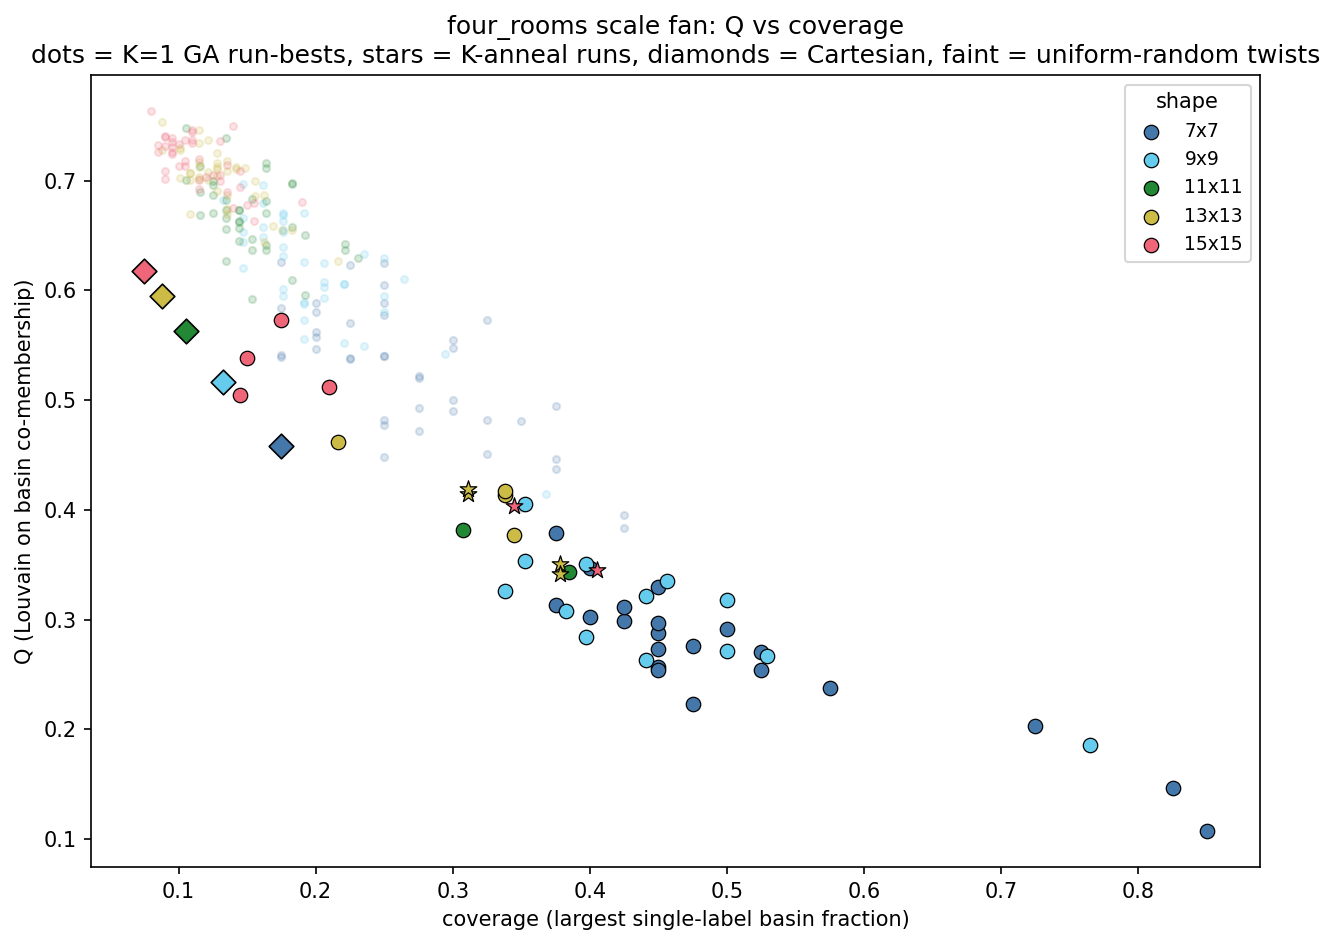
\includegraphics[width=0.72\textwidth]{F-q-vs-coverage-scale-fan.png}
  \caption[Structure manifold across scales]{\code{four\_rooms} twists on
  the coverage--modularity manifold across grid sides (colour), with
  uniform-random twists (faint), Cartesian (diamonds), full-goal
  run-bests (dots), and annealed runs (stars).  At $15 \times 15$ the
  fixed-budget full-goal cohort sits near the random end; the annealed
  runs sit deep in the consolidated-homing region the smaller scales
  occupy.}
  \label{fig:scale-fan}
\end{figure}

\section{Related work}
\label{sec:related}

% TODO: position against (i) fitness approximation / surrogate-assisted
% evolutionary computation; (ii) noisy fitness and implicit averaging in
% EAs; (iii) mini-batch stochastic gradient descent as the
% optimisation-community analogue (fresh mini-batch per step; small
% batches as implicit regularisation); (iv) simulated annealing (the
% schedule anneals selection NOISE rather than temperature).  Citations
% to be gathered; none currently in refs.bib.

\section{Discussion}
\label{sec:discussion}

The result is a recipe, and its two halves matter equally.  Evolve cheap
and noisy: a fresh $10\%$ goal batch per generation costs a tenth of the
true objective and explores more per unit of evaluation, because the
noise it injects at the top of the ranking prevents early entrenchment
--- attempts to remove that noise mid-run (Section~\ref{sec:j-harmful})
do measurable harm.  Then consolidate once: a short full-goal tail,
seeded with the whole final population rather than a champion, locks in
the found attractor --- and the pilot's identity analysis says
\emph{locks in} is the right phrase: same cycle, same home, most of the
genome already in place.

Why does the cheap stage find the right objects?  The fitness it
optimises is an unbiased estimate of the true objective whose variance
acts on selection, not on the landscape: the attractor structures that
make a twist good --- world-spanning basins draining to a compact home
--- help on \emph{most} goals, so they survive any batch, while genome
features that help only a few goals cannot hold their rank from batch to
batch.  Subsampling filters for exactly the goal-general structure the
research programme cares about.  This also bounds the recipe's scope: an
application whose value concentrates in a few critical goals would be
poorly served by uniform subsampling, and would want stratified or
importance-weighted batches instead.

Three continuations are queued.  Adaptive $K$ --- growing the batch as
the population converges --- would replace the hand-tuned two-stage
schedule with a self-scheduling one; the failure of elite re-evaluation
suggests any adaptation should act globally on $K$ rather than
selectively on ranking positions.  The $25 \times 25$ pair currently in
progress tests the schedule at a scale where full-goal evolution is
impractical outright: a single full-goal generation there costs what an
entire subsampled generation costs at ten times the batch.  And the
cache-plus-population handoff generalises to any staged curriculum ---
coarse-to-fine over goal sets, worlds, or fitness objectives --- wherever
the evaluation cache can be made stage-agnostic.

\printbibliography

\end{document}
